\documentclass[11pt, a4paper]{article}
\usepackage[letterpaper, portrait, margin=0.5in]{geometry}
\usepackage[english]{babel}  % force American English hyphenation patterns
\usepackage{amsmath,mathtools}

\usepackage{graphicx}
\usepackage{wrapfig}


\begin{document}
\title{Chapter 15 Periodic Motion}
\author{Apostolos Delis}
\date{\today}
\maketitle

\tableofcontents
\section[15.1, Types of Mechanical Wabves]{Types of Mechanical Waves}
\begin{itemize}
    \item A mechanical wave is a disturbance that travels through some material or
        substance called the medium for the wave.
    \item There are three varieties of mechanical waves

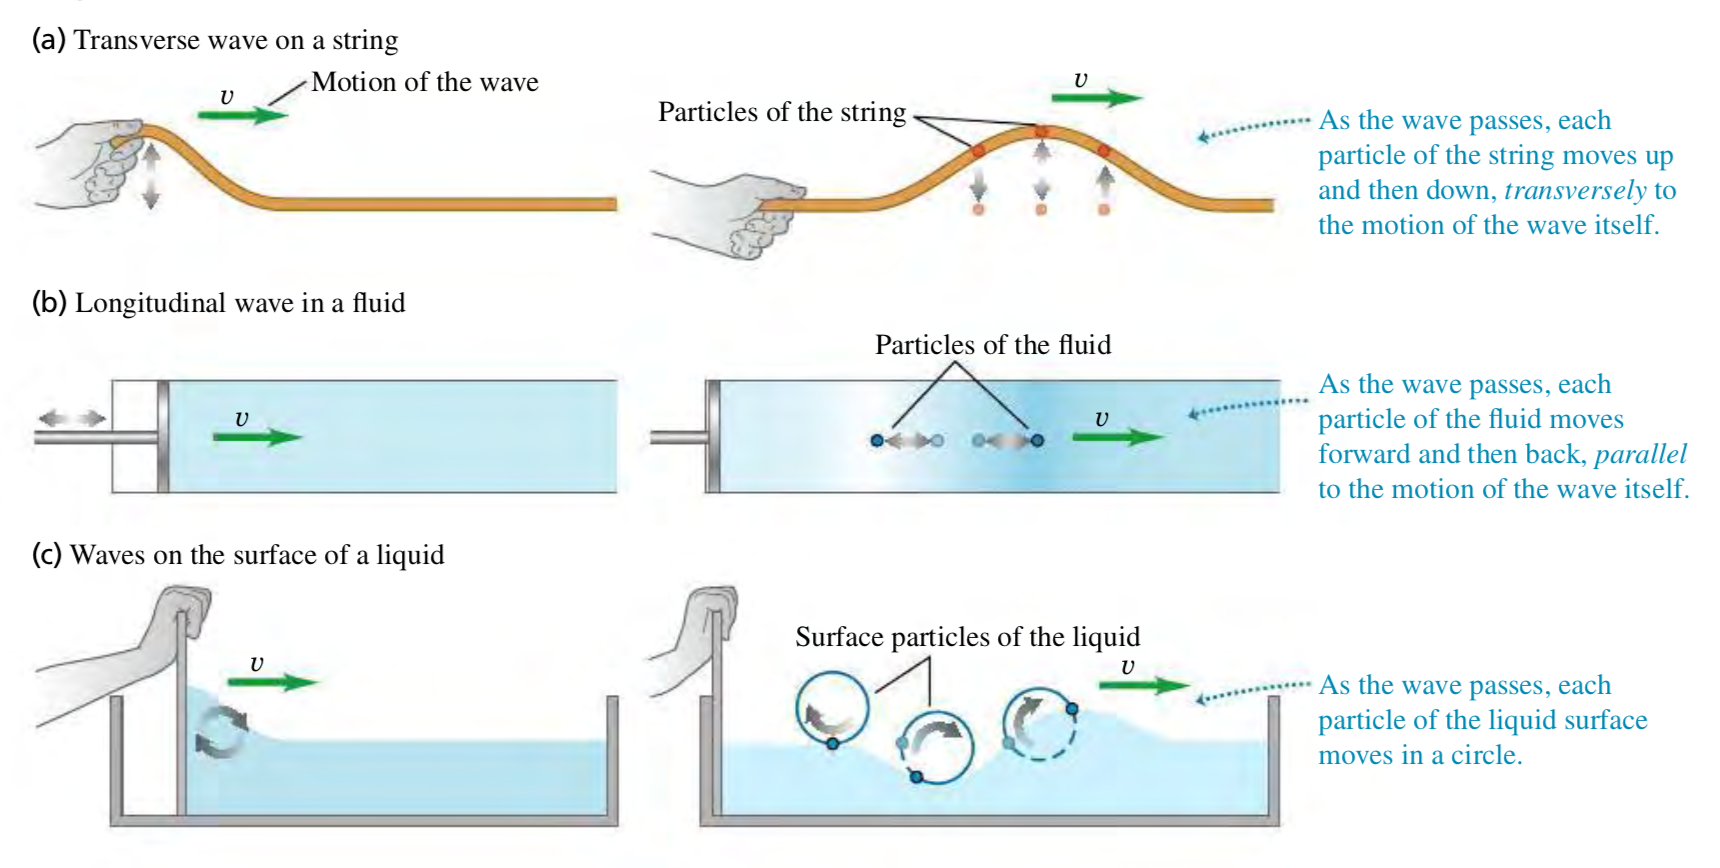
\includegraphics[scale=0.65]{images/mech_waves.png}

    \item Waves that have displacements of the medium perpendicular to to their direction
        of travel are called transverse waves while waves that have displacement in
        the direction of motion are called longitudinal waves
    \item Waves transport energy, not matter from one region to another
\end{itemize}

\section[15.2, Periodic Waves]{Periodic Waves}

\subsection{Periodic Tranverse Waves}

\begin{itemize}
    \item Suppose you move a string up and down with simple harmonic motion. The wave
        that results is a symmetric sequence of crests and troughs. These waves are
        called sinusoidal waves.
    \item for a periodic wave, the shape of the string at any instant is a repeating patterm, 
        where the length of that pattern is $\lambda$ 
    \item The speed of the wave is thus given by $v = \lambda/T$
\end{itemize}
\end{document}
